\documentclass[letterpaper]{article}
\usepackage{amsmath}
\usepackage{array}
\usepackage{color}
\usepackage{graphicx}
\usepackage{float} % utiliser H pour forcer a mettre l'image ou on veut
\usepackage{lscape} % utilisation du mode paysage
\usepackage{mathbbol} % permet d'avoir le vrai symbol pour les reels grace a mathbb
\usepackage{enumerate} % permet d'utiliser enumerate
\usepackage{moreverb} % permet d'utiliser verbatimtab : conservation la tabulation
\usepackage{stmaryrd} % permet d'utiliser \llbrackedt et \rrbracket : double crochet
\usepackage[noabbrev]{cleveref} % permet d'utiliser cref and Cref
\usepackage{caption} % permet d'utiliser subcaption
\usepackage{subcaption} % permet d'utiliser subfigure, subtable, etc
\usepackage[margin=1.in]{geometry} % controle les marges du document


\newcommand\bn{\boldsymbol{\nabla}}
\newcommand\bo{\boldsymbol{\Omega}}
\newcommand\br{\mathbf{r}}
\newcommand\la{\left\langle}
\newcommand\ra{\right\rangle}
\newcommand\bs{\boldsymbol}
\newcommand\red{\textcolor{red}}
\newcommand\ldb{\{\!\!\{}
\newcommand\rdb{\}\!\!\}}
\newcommand\llb{\llbracket}
\newcommand\rrb{\rrbracket}

\renewcommand{\(}{\left(}
\renewcommand{\)}{\right)}
\renewcommand{\[}{\left[}
\renewcommand{\]}{\right]}


\begin{document}
\title{Parallel Sweep on Adapted Mesh}
\author{Bruno Turcksin} 
\date{}
\maketitle

% In the paper, they gave a weight of 1/3 instead of zero to the arcs between
% two different processors.
\section{Introduction}
When using the discrete ordinates method \cite{} to discretize the transport equation,
it is customary to sweep through mesh \cite{}. Sweeping through a mesh can be
viewed as a resource-constrained project scheduling \cite{} (\red{talk more
about that}). In \cite{Adams2013}, a family of optimal sweeping algorithms is
described for regular grids. It is noticeable that such an important problem,
has been solved only recently for regular grids. For unstructured grids, several
algorithms have been proposed \cite{}. It is important to notice that the
optimal scheduling depends on the partitioning of the mesh. Two identical meshes
partitioned differently will lead to different optimal scheduling. Therefore the
interaction of sweeping and algorithm should be studied together. However, in
this paper, we will assume that the partitioning is given. This case covers the
case where partitioning is done by a third-party package \cite{} or the
partitioning cannot be tailored for the transport because others physics must be
accounted for. Here we will study a particular case of unstructured mesh namely
adaptively refined mesh \cite{}. In this paper, we study the CAP-PFB algorithm
introduced in \cite{Mo2014}. In particular, we will study how the algorithm
behaves on regular grids and how it can modified for mesh constructed using
adaptive mesh refinement (AMR). \red{Talk about deal.II and say that this is
only preliminary results -> no deal.II}

\section{Parallel sweeps on AMR mesh}
\subsection{CAP-PFB algorithm}
In this section, we explain the CAP-PFB (\red{extend}) introduced in
\cite{Mo2014}. The algorithm is based on the observation that when we try to
start the tasks as soon as possible, we have a lot of work at the beginning but
it trails off and to only few tasks later on. The opposite is true when we try
to start the tasks as late as possible, we have few tasks at the beginning but a
lot of work at the end. The idea of FP (\red{extend}) is to alternate forward
and backward iteration to have a lot of work all the time and thus, decrease the
time needed to execute all the tasks.
\subsection{CAP-PFB on adapted mesh}
In \cref{subdomain_id}, we show the partitioning of mesh using deal.II \cite{} and
p4est \cite{} on 16 processors. This is a typical mesh produced by these
libraries and it represents the case that we want to tackle. 
\begin{figure}[H]
  \begin{subfigure}[b]{.5\textwidth}
    \centering
    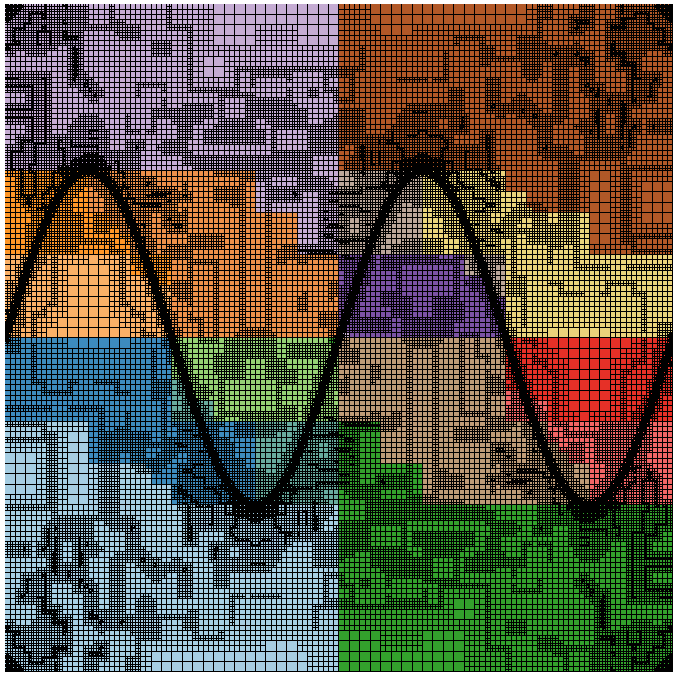
\includegraphics[width=5cm]{subdomain_id_0}
    \caption{Partitioning and mesh.}
  \end{subfigure}
  \begin{subfigure}[b]{.5\textwidth}
    \centering
    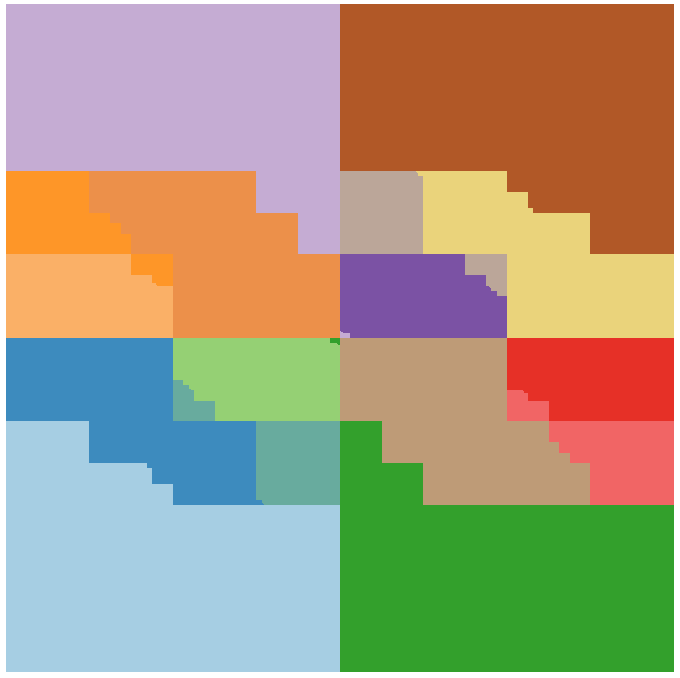
\includegraphics[width=5cm]{subdomain_id_1}
    \caption{Partitioning.}
  \end{subfigure}
  \caption{Partitioning and mesh using 16 processors for a typical problem
  (Step-40).}
  \label{subdomain_id}
\end{figure}
We can see that the domain owned by each processors are not convex and that some
processors own disjoint domains. In \cite{Mo2014}, the authors studied the case
where all the tasks have the same amount of work to do because the scheduling
algorithm will converge. This can be achieved by scheduling task that correspond
to only one cell. However, this will create an excessive amount of messages
which will negatively impact the performance \cite{}. Therefore, it is necessary
to have tasks that covers more than one cells. On a totally unstructured mesh,
gathering cells to form convex zones can be a hard problem. However, this can be
easily done on an AMR mesh, since the children of a coarse cell can be gather to
form a convex zone. It is of coarse necessary that all the children are owned by
the same processor. This process can be extended to grand-children,
great-grand-children, etc. This will create tasks that have very different
numbers of cells associated to them either because the cells have not been
refined as much as others or because some descendants of a cells are owned by
different processors. Having tasks containing different numbers of cells can be
taken into account in CAP-PFB but the resulting algorithm loses its convergence
property. 


\section{Results}
In this section, we look at the number of stages produced by the heuristic. In
the first test, we compared the sweep ordering produced by CAP-PFB with the
optimal solution. In the second test, we look at the ordering on an AMR mesh.
\subsection{Uniform mesh}
Uniform mesh $S_8$ (40 directions). Number of processors used: $10\times10=100$, 
$30\times30=900$, $50\times50=2500$, and $70\times70=4900$. For each test, we 
start with three different initial sweep ordering. From \cite{Adams2013}, we know
that the optimal number of stages on a 2D mesh is:
\begin{equation}
  \mu = P_x + P_y - 4 + N_{\textrm{task}},
\end{equation}
with $P_x \times P_y$ the process grid and $N_{\textrm{task}}$ the number of
tasks that each processors has to executed (40 in this example). Because CAP-PFB
is an heuristic that requires an initial scheduling, we use three different
initial scheduling for each tests.

\begin{table}[H]
  \begin{center}
    \begin{tabular}{|c|c|c|c|c|}
      \hline
      N. procs & Init. n. stages & Final n. stages & Optimal n. stages & Iter. \\
      \hline
      $10\times 10$ (no seed) &  580 &  56 &  56 & 1 \\
      $10\times 10$ (seed=0)  &  155 &  56 &  56 & 2 \\
      $10\times 10$ (seed=1)  &  153 &  56 &  56 & 1 \\
      $30\times 30$ (no seed) & 1780 &  96 &  96 & 1 \\
      $30\times 30$ (seed=0)  &  392 &  96 &  96 & 2 \\
      $30\times 30$ (seed=1)  &  376 &  96 &  96 & 2 \\
      $50\times 50$ (no seed) & 2980 & 136 & 136 & 1 \\
      $50\times 50$ (seed=0)  &  570 & 136 & 136 & 2 \\ % much faster than no
      % seed (less than one day instead of two)
      $50\times 50$ (seed=1)  &  573 & 136 & 136 & 2 \\
      $70\times 70$ (no seed) & & & 176 & \\
      $70\times 70$ (seed=0)  & & & 176 & \\
      $70\times 70$ (seed=1)  & & & 176 & \\
      \hline
    \end{tabular}
  \end{center}
\end{table}
where N. procs is the number of processors, Init. n. stages is the number of
stages of the initial scheduling, Final n. stages is the number of stages of the
final scheduling, Optimal n. stages is the number of stages of the optimal
scheduling, and Iter. is the number of CAP-FBS performed. We can see that the
heuristic converges to the optimal solution in only one or two iterations for
every initial scheduling.

\subsection{AMR mesh}

\subsection{AMR with discontinuous partitioning}

\section{Conclusions}


\bibliographystyle{unsrt}
\bibliography{database}

\end{document}

